%! TeX program = lualatex
\documentclass[a4paper,11pt]{article} 
% packages
\usepackage{fontspec}
\setmainfont{EB Garamond}
% for tironian et fallback
% % \directlua{luaotfload.add_fallback
% % ("emojifallback",
% %      {"Noto Serif:mode=harf"}
% % )}
% % \setmainfont{EB Garamond}[RawFeature={fallback=emojifallback}]

\setmonofont[Scale=MatchLowercase]{Deja Vu Sans Mono}
\usepackage[a4paper,left=2cm,right=2cm,top=\dimexpr15mm+1.5\baselineskip,bottom=2cm]{geometry}
\setlength{\parindent}{0pt}

\usepackage{fancyhdr}       % Headers and footers 
\fancyhead[R]{\normalfont \leftmark}
\fancyhead[L]{}
\pagestyle{fancy}

\usepackage{multicol}
\usepackage{microtype}      % Slightly tweak font spacing for aesthetics
\usepackage[english]{babel} % Language hyphenation and typographical rules
\usepackage[final, colorlinks = true, urlcolor = blue, linkcolor = black]{hyperref} 
\usepackage{changepage}     % adjust margins on the fly

\usepackage{minted}
\usemintedstyle{algol_nu}
\usepackage{xcolor}

\usepackage{pgfplots}
\pgfplotsset{width=\textwidth,compat=1.9}

\usepackage{caption}
\newenvironment{code}{\captionsetup{type=listing}}{}

\usepackage[yyyymmdd]{datetime}
\renewcommand{\dateseparator}{-}

\usepackage{titlesec}

\begin{document}
\begin{titlepage}
    \begin{center}
        \hrule
        \vspace*{0.6cm}
        \huge \textbf{CT331}
        \vspace*{0.6cm}
        \hrule
        \LARGE
       \vspace{0.5cm}
       PROGRAMMING PARADIGMS
       \vspace{0.5cm}
       \hrule
            
       \vfill
       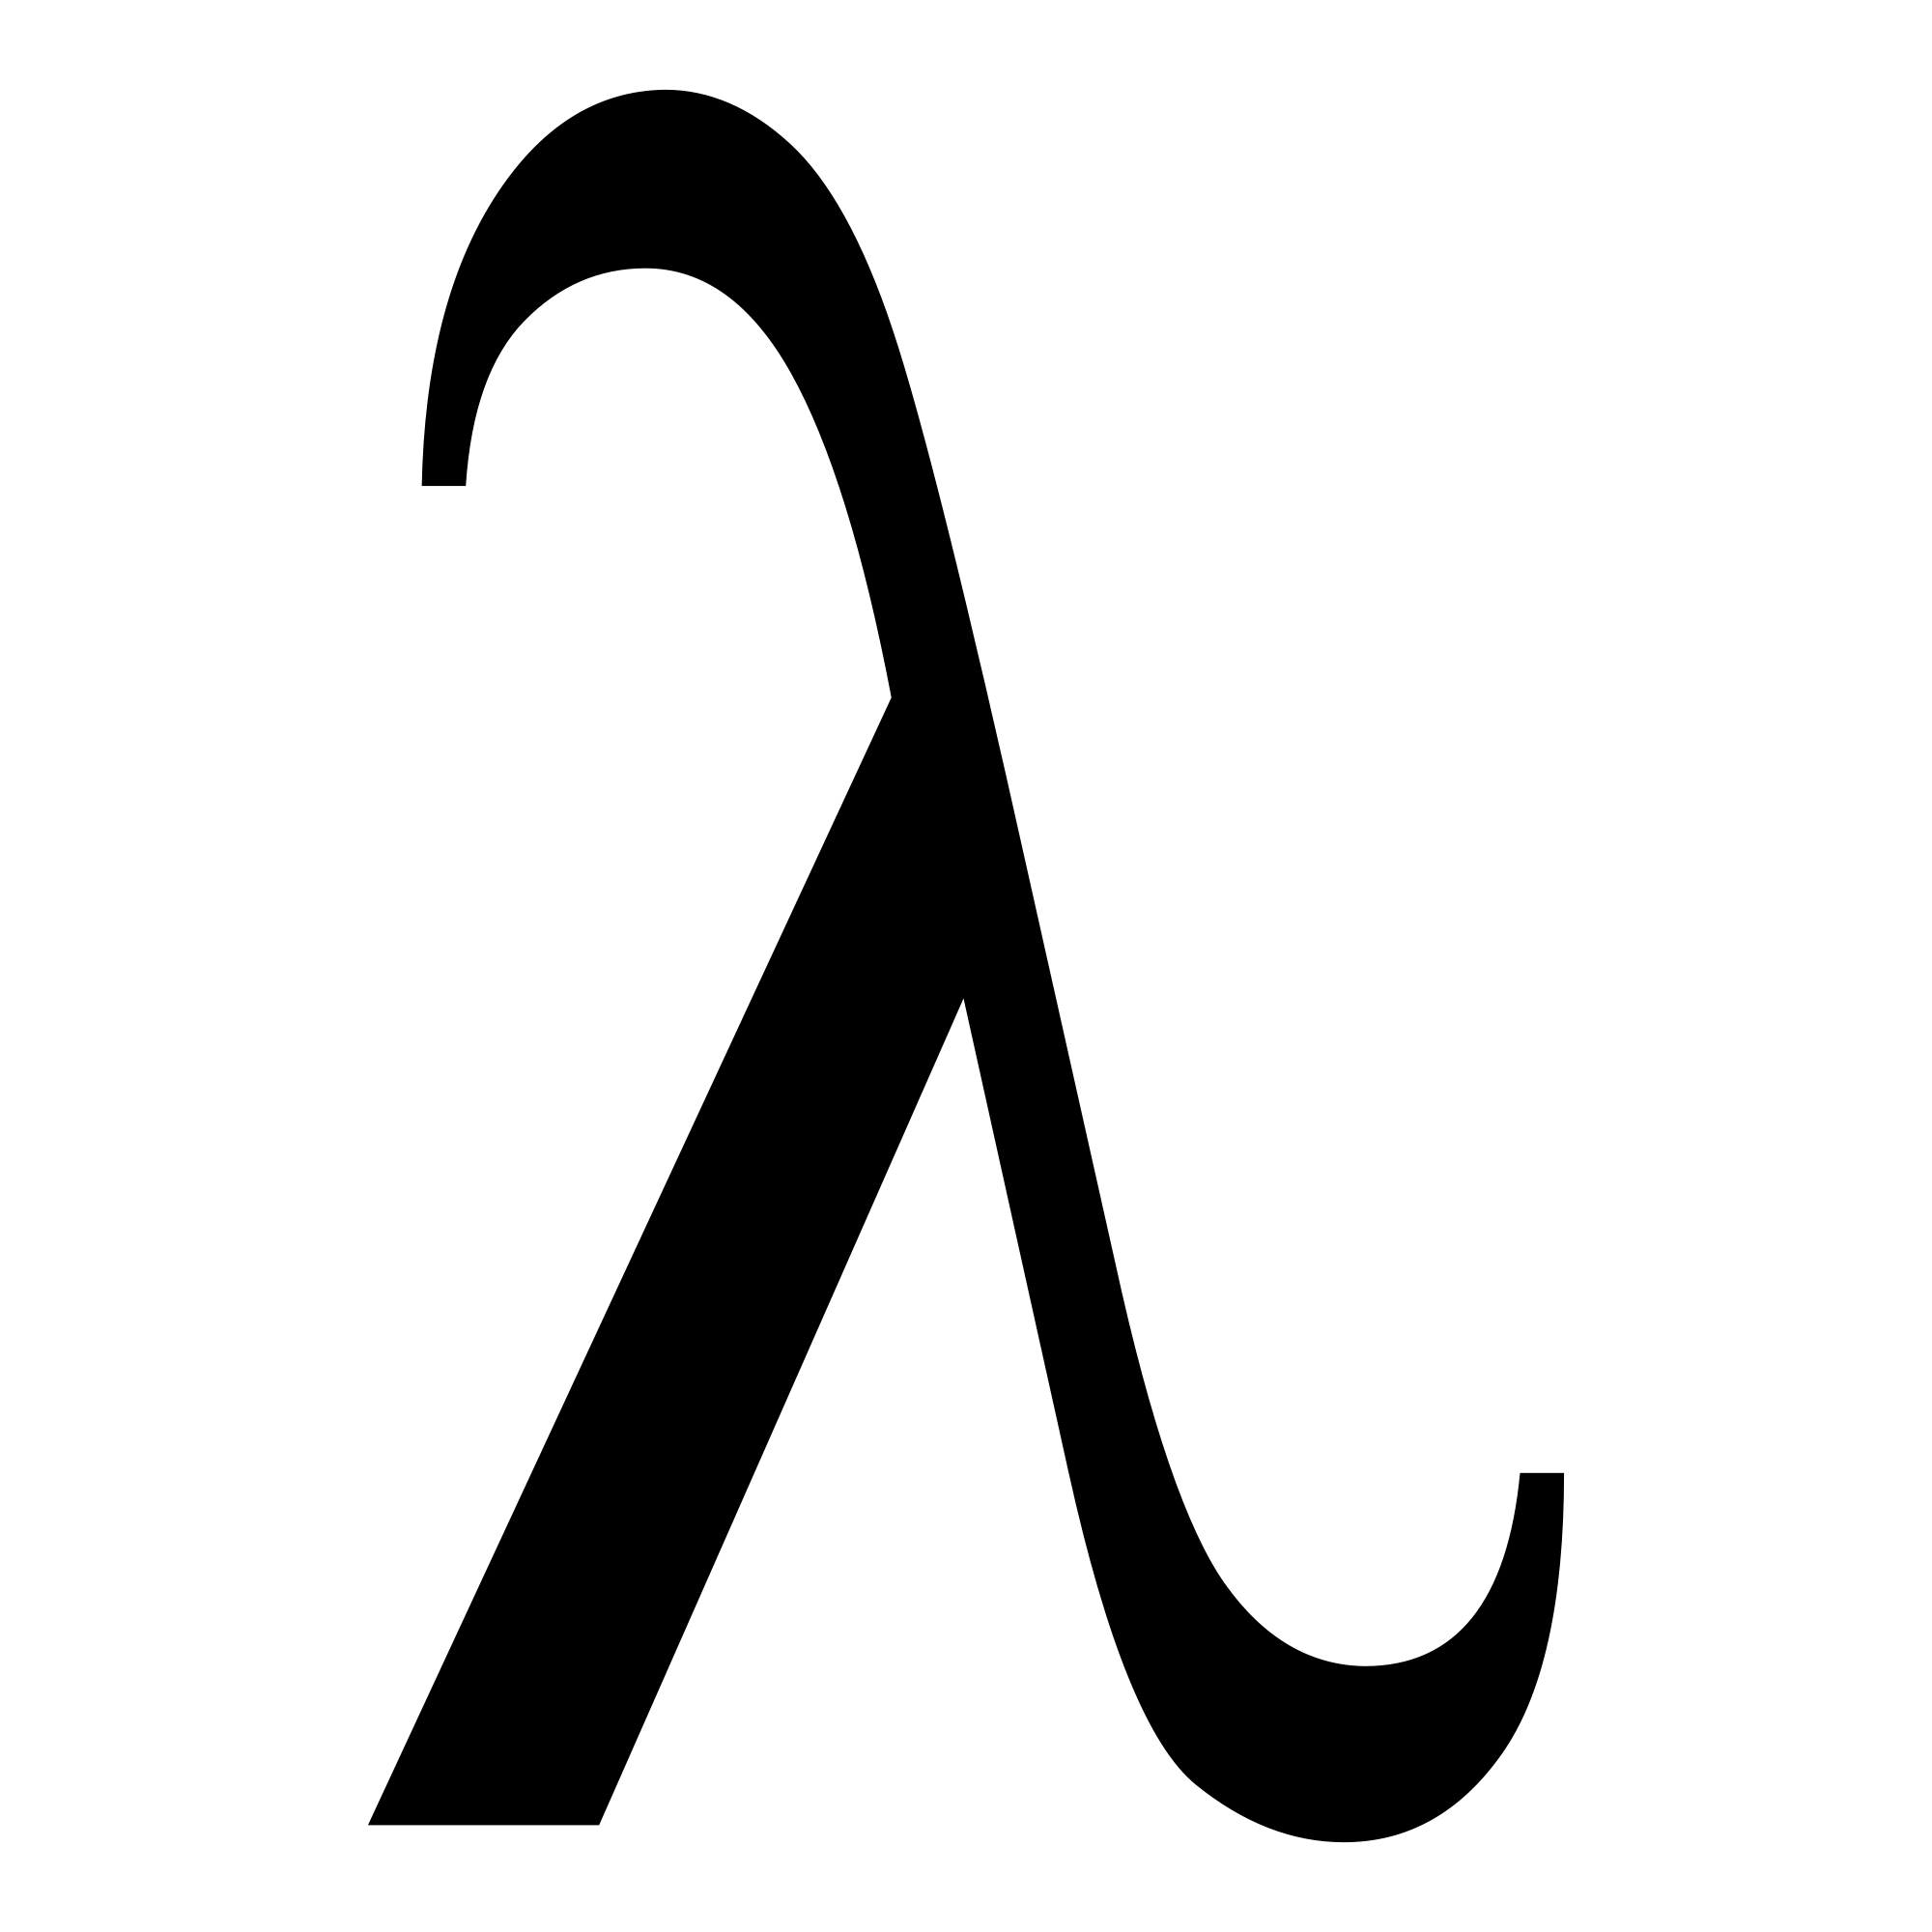
\includegraphics[width=0.8\textwidth]{images/lambda.png}
        \vfill

        \Large
       \vspace{0.5cm}
       \hrule
       \vspace{0.5cm}
       \textbf{Andreas Ó hAoḋa}
       % \vspace{0.5cm}
       % \hrule
       % \vspace{0.5cm}
            
       \normalsize
       University of Galway

       \today

       \vspace{0.5cm}
       \hrule
    \end{center}
\end{titlepage}

\pagenumbering{roman}
\newpage
\tableofcontents
\newpage
\setcounter{page}{1}
\pagenumbering{arabic}

\section{Introduction}
\subsection{Lecturer Contact Information}
\begin{itemize}
    \item   Finlay Smith, School of Computer Science. 
    \item   \href{mailto://finlay.smith@universityofgalway.ie}{\texttt{finlay.smith@universityofgalway.ie}}
\end{itemize}

\subsection{Syllabus}
This module introduces three different programming paradigms: Procedural, Functional \& Logical.
This will involve 3 programming languages: C (mostly function pointers - knowledge of C is assumed), LISP
(a functional language) and Prolog (a logical language).
Both LISP and Prolog will both be introduced but neither will be fully covered in this module.
There are no books required or recommended for this course. 

\subsubsection{Marking}
30\% of the marks for this module will be for the three assignments (one for each paradigm).
The remaining 70\% of the marks will be for the written exam.

\subsection{Programming Paradigms}
A \textbf{paradigm} is a typical example or pattern of something; a pattern or model. 
A \textbf{programming paradigm} is a pattern or model of programming.
Various types of programming languages are better suited to solving particular problems.
Programming language implementations  differ on semantics \& syntax:
\begin{itemize}
    \item   \textbf{Syntax} refers to the rules of the language; it allows us to form valid expressions \& statements.
    \item   \textbf{Semantics} refers to the meaning of those expressions \& statements.
\end{itemize}

Programming languages can be classified according to the features that they have with respect to both the conceptual \& implementation 
level.
An alternative definition for a \textbf{programming paradigm} is a collection of abstract features that categorise a group of 
languages.

``\textit{The popularity of a paradigm is due to one community deciding which problems are important to solve and then supporting the 
most promising paradigm for attacking these problems.}'' -- Thomas Kuhn.

\subsection{Influences on Paradigms}
\begin{itemize}
    \item   Computer Capabilities.
    \item   Applications. 
    \item   Programming Methods: Language designs have evolved to reflect changing understanding of good methods for writing 
            large \& complex programs. 
    \item   Implementation Methods: Early compilers to optimised compilers; structured engineering to software engineering; data 
            abstraction to OO.
    \item   Theoretical Studies: Formal maths methods have deepened our understanding of strengths \& weaknesses of language
            features and thus influenced the choice \& inclusion of those features. 
    \item   Standardisation (has proved to be a strong conservative influence on the evolution of programming language design).
\end{itemize}

\subsection{Why Learn Different Paradigms?}
\begin{itemize}
    \item   Different paradigms make different trade-offs; What's tricky in one paradigm is ``baked in''  in another.
    \item   Changing paradigms forces you to ``change gears''.
    \item   It will prepare you for learning languages that you've never heard of or that may not exist yet.
    \item   Helps you to decide what the best tool for the job is.
    \item   Helps you to understand languages at a deeper level.
\end{itemize}

\subsubsection{Why Learn Functional Programming?}
\begin{itemize}
    \item   It's one of the oldest paradigm (Lisp: 1958, still widely used today).
    \item   Heavily based on mathematical concepts (proofs, lambda calculations).
    \item   Elegant solutions (recursion).
    \item   Other paradigms can be interpreted in terms of functional programming.
\end{itemize}

\subsubsection{Why Learn Logical Programming?}
\begin{itemize}
    \item   Long history. 
    \item   ALlows implementation of things that are difficult in other paradigms.
    \item   \emph{Very} different
    \item   Helps to conceptualise logical problems.
\end{itemize}

\subsubsection{Why Learn Imperative Programming?}
\begin{itemize}
    \item   The oldest paradigm -- goes back as far as punch cards \& magnetic loops.
    \item   Much closer representation of how the machine actually works, i.e. ``closer to the metal''.
    \item   Can help to recognise optimisation issues / computational bottlenecks.
    \item   Contextualises many other systems (UNIX, Linux, etc.).
\end{itemize}

\subsubsection{Why Learn Object-Oriented Programming?}
\begin{itemize}
    \item   Tries to represent the real world.
    \item   Abstraction \& inheritance.
    \item   Object-Oriented is everywhere.
\end{itemize}

\section{Overview of Object-Oriented Programming}
Object-Oriented languages include:
\begin{multicols}{2}
\begin{itemize}
    \item   Java.
    \item   C\#.
    \item   VB.NET. 
    \item   Scala. 
    \item   JavaScript. 
    \item   Python.
    \item   PHP. 
    \item   Smalltalk.
    \item   Ruby.
\end{itemize}
\end{multicols}

\subsection{Fundamentals of Object-Oriented Programming}
\begin{itemize}
    \item   Everything is an object. 
    \item   Computation is performed by message-passing. 
    \item   Every \textbf{object} is an \textbf{instance} of a \textbf{class} which is a grouping of similar objects.
    \item   \textbf{Inheritance} describes the relationships between classes.
\end{itemize}

Object-Oriented Programming focuses on the objects that the program represents and allows them to exhibit ``behaviour''.

\subsection{Four Major Principles of OOP}
\subsubsection{Encapsulation}
Data is hidden as if \textbf{encapsulated} within the object. 
Direct access to the data is restricted, instead we use methods to get, set, \& manipulate data. 
Manipulation of data is hidden. 
The object caller doesn't need to know what's actually going on behind the scenes.
We can be (fairly) sure that nobody else is fiddling with our data.

\subsubsection{Abstraction}
Functionality can be defined without actually being implemented.
High-level interfaces provide method types/names without implementation. 
This allows case-specific implementation, allows one person to define the functionality \& another to implement, and
allows the representation to be changed without affecting ``public'' view of the class.
This is helpful when designing large systems. 

\subsubsection{Inheritance}
Classes can \textbf{inherit} functionality without re-implementing.
This prevents the duplication of code.
This is also helpful when designing large systems; it encourages a well-structured codebase.

\subsubsection{Polymorphism}
Objects of one class can be treated like objects of other classes.

\section{Imperative \& Procedural Programming}
\subsection{Imperative Programming}
\textbf{Imperative programming} involves telling the computer to perform a set of actions, one after the other. 
Most programming languages have imperative aspects.
Imperative programming consists of a list of instructions, \verb|GOTO| statements, and little or no structure.
E.g., Assembly.

\subsection{Procedural Progamming}
\textbf{Procedural progamming} splits actions into \textbf{procedures} or tasks. 
Procedures can be made up of other procedures (composition, recursion). 
The code is structured, uses ``functions'' or procedures, encourages code re-use, and encourages encapsulation \&
composition.
Note that procedural functions are not to be confused with Functional Programming.

\subsubsection{Structured Programming}
Examples of structured programming languages include basically everything except Assembly.
\begin{itemize}
    \item   Code is structured.
    \item   \verb|while|, \verb|for|, \verb|if|, \verb|else,| \verb|switch|, \verb|class|, \verb|function|, etc.
    \item   Less emphasis on \verb|GOTO| statements.
    \item   Creating a structure to manage instructions.
    \item   Allows more complex programs to be built.
    \item   Easier to understand.
    \item   Helps to avoid \verb|GOTO| bugs \& spaghetti code.
\end{itemize}

\subsection{The C Programming Language}
\textbf{C} is a procedural, imperative, structured ``systems language''.
It came into being around 1969-1973 in parallel with the development of the UNIX operating system.
Basic Compiled Programming Language (BCPL) \rightarrow B \rightarrow C...
C has had an ANSI standard since the 1980s.
Now one of the most popular \& powerful languages in use today.
\begin{code}
\begin{minted}[texcl, mathescape, linenos, breaklines, frame=single]{c}
// header inclusion: functionally defined in stdio.h is added into the program by the compiler, specifically the Linker step of the compiler
// "stdio" is short for "Standard Input / Output"
#include <stdio.h> 

// function prototype: tells the compiler that the function exists before it has been implemented
// allows the compiler to handle recursion, or functions calling each other
void sayHello(); 

// function definition: implements the function 
// note: data type, arguments, return
void sayHello() {
    // calling a function: printf takes a char* argument
    printf("Hello World!\n");
}

// main function: the entry point to the progam
// returns int
// takes two arguments: argc (the number of command-line arguments) & argv (an array of the arguments)
int main(int argc, char* argv[]) {
    // calling a function: sayhello takes no argument. nothing is returned
    sayHello();
    return 0;
}
\end{minted}
\caption{Example C Program: \texttt{helloWorld.c}}
\end{code}

\begin{code}
\begin{minted}[texcl, mathescape, linenos, breaklines, frame=single]{c}
#include <stdio.h> 

int add(int a, int b); 

int add(int a, int b) {
    return a+b; 
}

int main(int argc, char* argv[]) {
    printf("Let's add some numbers...\n"); 
    int first = 8; 
    int second = 4; 
    printf("The first number is %d\n", first);
    printf("The second number is %d\n", second);

    // "add" is a function that returns an int
    // the returned int is stored in the "result" variable - they must have the same data type
    int result = add(first, second);


    // "%d" is for ints - strictly decimal ints 
    // "%i" is any int including octal and hexadecimal 
    printf("When we add them together we get: %d\n", result);

    return 0;
}

\end{minted}
\caption{Example C Program: \texttt{addNumbers.c}}
\end{code}

\subsubsection{Pointers}
\begin{minted}[texcl, mathescape, linenos, breaklines, frame=single]{c}
int* p; // variable p is a pointer to an integer value
int i;  // integer value
\end{minted}

You can \textbf{dereference} a pointer into a value with \verb|*|. 
\begin{minted}[texcl, mathescape, linenos, breaklines, frame=single]{c}
// ineger i2 is assigned the integer value that the pointer p is pointing to 
int i2 = *p;
\end{minted}
 
You can get a pointer to a value with \verb|&|. 
\begin{minted}[texcl, mathescape, linenos, breaklines, frame=single]{c}
// pointer p2 points to the address of integer i
int* p2 = &i;
\end{minted}

A function effectively breaking the convention that arguments are not changed in a function is a \textbf{side effect}. 
This is done by passing addresses.
\begin{minted}[texcl, mathescape, linenos, breaklines, frame=single]{c}
#include<stdio.h>

void swap(int* x, int* y) {
    int temp = *x; 
    *x = *y; 
    *y = temp;
}

int main(int argc, char* arv[]) {
    int a = 8; 
    int b = 4;
    swap(&a, &b);   // this should make a=4 & b=8
}
\end{minted}

\subsubsection{Arrays \& Pointers}
\begin{minted}[texcl, mathescape, linenos, breaklines, frame=single]{c}
int intArr[5];  // an integer array of size 5
// intArr is a pointer to the 0th element of the array - the same as &intArr[0]

intArr[2] = 3;  // same as *(intArr+2) = 3;
// (intArr + 2) is of type (int*) while intArr[2] is of type int
// in the latter case, the pointer is dereferenced
// (intArr + 2) is the same as (&(intArr[2]))
// note that the + operator here is not simple addition - it moves the pointer by the size of the type
\end{minted}

\subsubsection{Generic Swap function?}
What about a swap function that works on any data type? 
\begin{code}
\begin{minted}[texcl, mathescape, linenos, breaklines, frame=single]{c}
void swap(void* x, void* y) {
    void temp = *x; // won't work!
    // we don't know what size data *x points to, so void temp can't work 
    // it is impossible to have a variable of type void for this reason 
    // but we can have a pointer of type void*

    *x = *y; 
    *y = temp;
}
\end{minted}
\caption{(Non-functional) Attempt at a Generic \texttt{swap} Function}
\end{code}
\mintinline{c}{void*} is a specific pointer type which points to some location in memory. 
It has no specific type and therefore no specific size.
\\\\
\mintinline{c}{sizeof(<type>)} returns the size in bytes of the object representation of \verb|<type>|.
\verb|sizeof()| is built-in to the C langauge.
\\\\
\mintinline{c}{void* memcpy(void* to, const void* from, size_t size)}. 
The \verb|memcpy()| function copies \verb|size| number of bytes from the object beginning at location \verb|from| into 
the object beginning at location \verb|to|. 
The value returned by \verb|memcpy()| is the value of \verb|to|. 
The \verb|memcpy()| function is defined in \verb|string.h|.

\begin{code}
\begin{minted}[texcl, mathescape, linenos, breaklines, frame=single]{c}
#include <string.h>

void generic_swap(void* vp1, void* vp2, int size) {
    char temp_buff[size];   // need malloc?
    memcpy(temp_buff, vp1, size);
    memcpy(vp1, vp2, size);
    memcpy(vp2, temp_buff, size);
}
\end{minted}
\caption{Generic Swap Function}
\end{code}

\subsection{Stacks vs Heaps}
A \textbf{stack} is a LIFO data structure of limited size \& limited access.
It supports only two operations: PUSH \& POP.
Stacks are very fast.
The limited size of stacks can result in stack overflow, and you cannot free memory in a stack except by POPping.
To continue the \verb|swap()| function from above:
\begin{minted}[texcl, mathescape, linenos, breaklines, frame=single]{c}
// first, a, b, & c are pushed onto the stack
char a = 'a';
int b = 100;
int c = 50;

// when swap() is called, x, y, & temp are pushed onto the stack
void swap(int* x, int* y) {
    int temp = *x;
    *x = *y;
    *y = temp;

    // when swap returns, x, y, & temp are popped from the stack and \textbf{their memory is no longer in use}
}

swap(b, c);
\end{minted}

But what if we want to keep track of \verb|temp| and use it later?
\\\\ 
A \textbf{heap} is an unordered data structure of (theoretically) unlimited size and global access. 
The heap operations are allocate \& free.
Heaps are slower than stacks.
Heaps are also harder to manage than stacks as they can get memory leaks.
\begin{minted}[texcl, mathescape, linenos, breaklines, frame=single]{c}
// first, b & c are pushed onto the stack
int b = 100;
int c = 50;

// when swap() is called, x, y, & temp are pushed onto the stack
void* swap(int* x, int* y) {
    int temp = *x;

    // we allocate space in memory to perm using malloc
    int* perm = malloc(int);
    perm = &temp;
    x = y;
    y = *perm;

    // when swap returns, x, y, & temp are popped from the stack
    // the memory allocated to perm is still in use 
    return perm;
}


void* p = swap(b, c);
free(p);
\end{minted}

Why not just return \verb|temp| in the same way?
\begin{itemize}
    \item   Even when this function terminates, another function can access perm using that pointer.
    \item   If we need to store a large or undeterminable amount of data, we can safely use the heap as there is no risk 
            of stack overflow and no risk of losing reference or accidental de-allocation of memory.
\end{itemize}

\section{Dynamic Memory}
FINISH OFF

\section{Functional Programming}
Given the same problem to solve, a program for said problem in any programming language can be considered 
equivalent to any other at the machine level in that the programs will result in changes to values contained in 
memory cells. 
However, there can be quite significant differences at both the conceptual \& implementation level.

\subsection{Lisp, Racket, \& Scheme}
\textbf{LISP} (more commonly referred to as \textbf{Lisp}) is a contraction of \textbf{List Processing}.
\textbf{Scheme} is a dialect of Lisp, and \textbf{Racket} is an implementation of Scheme.
Lisp uses prefix  (Polish) notation, e.g.: \verb|(+ 3 4)|, \verb|(* 5 6)|, \verb|(- 4 (* 5 6))|, etc.

\subsubsection{Function vs Literal}
Parentheses are used to represent a \textbf{function}:
\begin{minted}[texcl, mathescape, linenos, breaklines, frame=single]{lisp}
(+ 3 4)         ; =   7
(* 5 6)         ; =  30
(- 4 (* 5 6))   ; = -26
\end{minted}

A single quote is used to represent a \textbf{literal}:
\begin{minted}[texcl, mathescape, linenos, breaklines, frame=single]{lisp}
(+ 3 4)     ; = 7
'(+ 3 4)    ; = '(+ 3 4)
\end{minted}

Rather than considering \verb|+| as the name of a function, the quote means to take everything literally, i.e. 
``\verb|+|'' is just a word.
Nothing is evaluated.

\subsubsection{S-Expressions}
Both code \& data are structured as nested lists in Lisp. 
\textbf{Symbolic Expressions} or s-expressions, sexprs, or sexps are a notation for nested list structures.
They are defined with a very simple recursive grammar, but produce a very flexible framework for computing.
An s-expression is defined as: 
\begin{enumerate}
    \item   An \textbf{atom}. 
            Atoms are considered to be ``indivisible''. 
            Primitive data types like numbers, strings, booleans, etc. are atoms. 
            Lists \& pairs (s-expressions) are not.
    \item   An expression in the form \verb|(X . Y)|, where \verb|X| \& \verb|Y| are s-expressions.
\end{enumerate}

A \textbf{pair} is two pieces of data together.
They are created by the \verb|cons| function, which is short for ``construct'', e.g. \verb|(cons 1 2)|.
The two values joined with \verb|cons| are printed between parentheses interspaced by a \verb|.| (a period): 
\begin{minted}[texcl, mathescape, breaklines, frame=single]{lisp}
> (cons "banana" "split")
'("banana" . "split")'
\end{minted}

\subsection{Lists}
A \textbf{list} is an ordered group of data.
List elements are separated by a space.
The list syntax is a shorthand for an s-expression.
Lists are displayed between parentheses using the \verb|'| (single quote character).
\begin{minted}[texcl, mathescape, breaklines, frame=single]{lisp}
'(1 2 3)                        ; list of numbers
'("this" "that" "the other")    ; list of strings
'(1 2 "three" 4)                ; list of mixed data types
\end{minted}

Lisp uses nested lists (which are essentially linked lists). 
We can access the first element of a list using the \verb|car| function:
\begin{minted}[texcl, mathescape, breaklines, frame=single]{lisp}
> (car '(1 2 3))
1
\end{minted}

We can access the rest of the list using the \verb|cdr| function:
\begin{minted}[texcl, mathescape, breaklines, frame=single]{lisp}
> (cdr '(1 2 3))
'(2 3)
\end{minted}

\verb|cdr| is analogous to \verb|element->rest| in our C linked list.
\begin{minted}[texcl, mathescape, breaklines, frame=single]{lisp}
> (car (cdr '(1 2 3)))
2
\end{minted}

There is a shorthand for a combination of \verb|car|s \& \verb|cdr|s (up to 4 operations usually but it depends 
on the Scheme environment), where  \verb|*| is \verb|a| or \verb|d| or a combination (if supported). 
For example, write a sequence of \verb|car|s \& \verb|cdr|s to extract: ``\verb|d|'' from list
\verb|(a b c d e f)| named \verb|lis|:
\begin{minted}[texcl, mathescape, linenos, breaklines, frame=single]{lisp}
;;;; these two are equivalent
(car (cdr (cdr (cdr  lis))))
cadddr(lis)
\end{minted}

Lists are really just \verb|cons| pairs where these second element is another list or \verb|empty|;
\verb|empty| is a special word, similar to \verb|NULL| in other languages.
\begin{minted}[texcl, mathescape, breaklines, frame=single]{lisp}
> (cons 2 empty)
'(2)

> (cons 1 (cons 2 empty))
'(1 2)
\end{minted}

The built-in functions \verb|list| \& \verb|append| provide a more convenient way to create lists.

\subsubsection{\texttt{define}}
\textbf{\texttt{define}} binds a variable to some data. 
Its format is \mintinline{lisp}{(define variable value)}.
\verb|define| is used for user-defined functions.
Note that user-defined functions can be used within other use defined functions as long as the functions are 
defined before they are invoked.
\begin{minted}[texcl, mathescape, linenos, breaklines, frame=single]{lisp}
(define (function_name parameter-list)
    Function-body
)

;;; calculates the absolute addition of two numbers where the function abs returns the absolute value of a number
(define (sumabs num1 num2) 
    (+ (abs num1) (abs num2)) 
)
\end{minted}
\begin{minted}[texcl, mathescape, breaklines, frame=single]{lisp}
> (sumabs 2 -3)
5
\end{minted}

\subsubsection{\texttt{list} \& \texttt{append}}
The \verb|list| function constructs a list from components. 
It takes the form \mintinline{lisp}{(list el-1 el-2 el-n)}. 
These components can be symbols, numbers, or lists.
\\\\
\verb|append| collects components from several lists into one list. 
Its arguments must be lists. 
\verb|append| takes the form \mintinline{lisp}{(append list1 list2 listn)}.



\end{document}
